\batchmode
\documentclass[twoside]{book}

% Packages required by doxygen
\usepackage{fixltx2e}
\usepackage{calc}
\usepackage{doxygen}
\usepackage[export]{adjustbox} % also loads graphicx
\usepackage{graphicx}
\usepackage[utf8]{inputenc}
\usepackage{makeidx}
\usepackage{multicol}
\usepackage{multirow}
\PassOptionsToPackage{warn}{textcomp}
\usepackage{textcomp}
\usepackage[nointegrals]{wasysym}
\usepackage[table]{xcolor}

% Font selection
\usepackage[T1]{fontenc}
\usepackage[scaled=.90]{helvet}
\usepackage{courier}
\usepackage{amssymb}
\usepackage{sectsty}
\renewcommand{\familydefault}{\sfdefault}
\allsectionsfont{%
  \fontseries{bc}\selectfont%
  \color{darkgray}%
}
\renewcommand{\DoxyLabelFont}{%
  \fontseries{bc}\selectfont%
  \color{darkgray}%
}
\newcommand{\+}{\discretionary{\mbox{\scriptsize$\hookleftarrow$}}{}{}}

% Page & text layout
\usepackage{geometry}
\geometry{%
  a4paper,%
  top=2.5cm,%
  bottom=2.5cm,%
  left=2.5cm,%
  right=2.5cm%
}
\tolerance=750
\hfuzz=15pt
\hbadness=750
\setlength{\emergencystretch}{15pt}
\setlength{\parindent}{0cm}
\setlength{\parskip}{3ex plus 2ex minus 2ex}
\makeatletter
\renewcommand{\paragraph}{%
  \@startsection{paragraph}{4}{0ex}{-1.0ex}{1.0ex}{%
    \normalfont\normalsize\bfseries\SS@parafont%
  }%
}
\renewcommand{\subparagraph}{%
  \@startsection{subparagraph}{5}{0ex}{-1.0ex}{1.0ex}{%
    \normalfont\normalsize\bfseries\SS@subparafont%
  }%
}
\makeatother

% Headers & footers
\usepackage{fancyhdr}
\pagestyle{fancyplain}
\fancyhead[LE]{\fancyplain{}{\bfseries\thepage}}
\fancyhead[CE]{\fancyplain{}{}}
\fancyhead[RE]{\fancyplain{}{\bfseries\leftmark}}
\fancyhead[LO]{\fancyplain{}{\bfseries\rightmark}}
\fancyhead[CO]{\fancyplain{}{}}
\fancyhead[RO]{\fancyplain{}{\bfseries\thepage}}
\fancyfoot[LE]{\fancyplain{}{}}
\fancyfoot[CE]{\fancyplain{}{}}
\fancyfoot[RE]{\fancyplain{}{\bfseries\scriptsize Generated by Doxygen }}
\fancyfoot[LO]{\fancyplain{}{\bfseries\scriptsize Generated by Doxygen }}
\fancyfoot[CO]{\fancyplain{}{}}
\fancyfoot[RO]{\fancyplain{}{}}
\renewcommand{\footrulewidth}{0.4pt}
\renewcommand{\chaptermark}[1]{%
  \markboth{#1}{}%
}
\renewcommand{\sectionmark}[1]{%
  \markright{\thesection\ #1}%
}

% Indices & bibliography
\usepackage{natbib}
\usepackage[titles]{tocloft}
\setcounter{tocdepth}{3}
\setcounter{secnumdepth}{5}
\makeindex

% Hyperlinks (required, but should be loaded last)
\usepackage{ifpdf}
\ifpdf
  \usepackage[pdftex,pagebackref=true]{hyperref}
\else
  \usepackage[ps2pdf,pagebackref=true]{hyperref}
\fi
\hypersetup{%
  colorlinks=true,%
  linkcolor=blue,%
  citecolor=blue,%
  unicode%
}

% Custom commands
\newcommand{\clearemptydoublepage}{%
  \newpage{\pagestyle{empty}\cleardoublepage}%
}

\usepackage{caption}
\captionsetup{labelsep=space,justification=centering,font={bf},singlelinecheck=off,skip=4pt,position=top}

%===== C O N T E N T S =====

\begin{document}

% Titlepage & ToC
\hypersetup{pageanchor=false,
             bookmarksnumbered=true
            }
\pagenumbering{alph}
\pagenumbering{arabic}
\hypersetup{pageanchor=true}

%--- Begin generated contents ---
\chapter{Demo problem\+: Flow of a fluid film down an inclined plane}
\label{index}\hypertarget{index}{}\hypertarget{index_q}{}\section{A few quick questions...}\label{index_q}
Since {\ttfamily oomph-\/lib} is developed as open-\/source software, any evidence that the code is being downloaded and used is very helpful for us as it helps to justify our continued work on this project.

We would therefore be extremely grateful if you could provide the information requested in the form below. Pressing the \char`\"{}submit\char`\"{} button will get you to the actual download page.

{\bfseries Note\+:} 
\begin{DoxyItemize}
\item All information will be treated as confidential. 
\item If you provide your email address and check the appropriate box we will add you to our mailing list to inform you of upgrades and bug fixes to the code. Rest assured that the mailing list is {\bfseries very low volume} -- we have better things to do than to bombard you with email. 
\item If you still feel reluctant to provide any of the information requested, feel free to enter some dummy input. The form will check that {\bfseries some} information has been entered but entering your name as \char`\"{}\+Joe Cool\char`\"{} is perfectly acceptable -- this is to discourage people from not providing the information simply because they are too lazy to type... 
\end{DoxyItemize}



 







 

 \hypertarget{index_pdf}{}\section{P\+D\+F file}\label{index_pdf}
A \href{../latex/refman.pdf}{\tt pdf version} of this document is available. \end{document}

\chapter{Namespace Index}
\section{Namespace List}
Here is a list of all namespaces with brief descriptions\+:\begin{DoxyCompactList}
\item\contentsline{section}{\hyperlink{namespaceGlobal__Physical__Variables}{Global\+\_\+\+Physical\+\_\+\+Variables} \\*Global variables that represent physical properties }{\pageref{namespaceGlobal__Physical__Variables}}{}
\item\contentsline{section}{\hyperlink{namespaceoomph}{oomph} }{\pageref{namespaceoomph}}{}
\item\contentsline{section}{\hyperlink{namespacePhysical__Variables}{Physical\+\_\+\+Variables} \\*Namespace for the solution of 2D linear shell equation }{\pageref{namespacePhysical__Variables}}{}
\end{DoxyCompactList}

\chapter{Hierarchical Index}
\section{Class Hierarchy}
This inheritance list is sorted roughly, but not completely, alphabetically\+:\begin{DoxyCompactList}
\item Problem\begin{DoxyCompactList}
\item \contentsline{section}{Unstructured\+Solid\+Problem$<$ E\+L\+E\+M\+E\+NT $>$}{\pageref{classUnstructuredSolidProblem}}{}
\end{DoxyCompactList}
\end{DoxyCompactList}

\chapter{Class Index}
\section{Class List}
Here are the classes, structs, unions and interfaces with brief descriptions\+:\begin{DoxyCompactList}
\item\contentsline{section}{\hyperlink{classPMLProblem}{P\+M\+L\+Problem$<$ E\+L\+E\+M\+E\+N\+T $>$} }{\pageref{classPMLProblem}}{}
\item\contentsline{section}{\hyperlink{classGlobalParameters_1_1TestPMLMapping}{Global\+Parameters\+::\+Test\+P\+M\+L\+Mapping} }{\pageref{classGlobalParameters_1_1TestPMLMapping}}{}
\end{DoxyCompactList}

\chapter{File Index}
\section{File List}
Here is a list of all files with brief descriptions\+:\begin{DoxyCompactList}
\item\contentsline{section}{\hyperlink{jeffery__orbit_8cc}{jeffery\+\_\+orbit.\+cc} }{\pageref{jeffery__orbit_8cc}}{}
\item\contentsline{section}{\hyperlink{jeffery__orbit_8txt__doxygenified_8h}{jeffery\+\_\+orbit.\+txt\+\_\+doxygenified.\+h} }{\pageref{jeffery__orbit_8txt__doxygenified_8h}}{}
\item\contentsline{section}{\hyperlink{my__taylor__hood__elements_8h}{my\+\_\+taylor\+\_\+hood\+\_\+elements.\+h} }{\pageref{my__taylor__hood__elements_8h}}{}
\end{DoxyCompactList}

\chapter{Namespace Documentation}
\hypertarget{namespaceGlobal__Physical__Variables}{}\section{Global\+\_\+\+Physical\+\_\+\+Variables Namespace Reference}
\label{namespaceGlobal__Physical__Variables}\index{Global\+\_\+\+Physical\+\_\+\+Variables@{Global\+\_\+\+Physical\+\_\+\+Variables}}


Namespace for physical parameters.  


\subsection*{Functions}
\begin{DoxyCompactItemize}
\item 
Vector$<$ double $>$ \hyperlink{namespaceGlobal__Physical__Variables_afae321364975eb56688ad13abc8ed6b7}{Gravity} (2)
\begin{DoxyCompactList}\small\item\em Gravity vector. \end{DoxyCompactList}\item 
void \hyperlink{namespaceGlobal__Physical__Variables_a87da705b8a46bed337cf5dbdd788b87b}{body\+\_\+force} (const double \&time, const Vector$<$ double $>$ \&x, Vector$<$ double $>$ \&result)
\begin{DoxyCompactList}\small\item\em Functional body force. \end{DoxyCompactList}\item 
void \hyperlink{namespaceGlobal__Physical__Variables_a9780d615ae07c4e00a436ab2973b54e6}{zero\+\_\+body\+\_\+force} (const double \&time, const Vector$<$ double $>$ \&x, Vector$<$ double $>$ \&result)
\begin{DoxyCompactList}\small\item\em Zero functional body force. \end{DoxyCompactList}\end{DoxyCompactItemize}
\subsection*{Variables}
\begin{DoxyCompactItemize}
\item 
double \hyperlink{namespaceGlobal__Physical__Variables_ab814e627d2eb5bc50318879d19ab16b9}{Re} =100
\begin{DoxyCompactList}\small\item\em Reynolds number. \end{DoxyCompactList}\item 
double \hyperlink{namespaceGlobal__Physical__Variables_ab1a845a672b4d74b304639a976dc65c6}{Re\+\_\+inv\+Fr} =100
\begin{DoxyCompactList}\small\item\em Reynolds/\+Froude number. \end{DoxyCompactList}\end{DoxyCompactItemize}


\subsection{Detailed Description}
Namespace for physical parameters. 

\subsection{Function Documentation}
\mbox{\Hypertarget{namespaceGlobal__Physical__Variables_a87da705b8a46bed337cf5dbdd788b87b}\label{namespaceGlobal__Physical__Variables_a87da705b8a46bed337cf5dbdd788b87b}} 
\index{Global\+\_\+\+Physical\+\_\+\+Variables@{Global\+\_\+\+Physical\+\_\+\+Variables}!body\+\_\+force@{body\+\_\+force}}
\index{body\+\_\+force@{body\+\_\+force}!Global\+\_\+\+Physical\+\_\+\+Variables@{Global\+\_\+\+Physical\+\_\+\+Variables}}
\subsubsection{\texorpdfstring{body\+\_\+force()}{body\_force()}}
{\footnotesize\ttfamily void Global\+\_\+\+Physical\+\_\+\+Variables\+::body\+\_\+force (\begin{DoxyParamCaption}\item[{const double \&}]{time,  }\item[{const Vector$<$ double $>$ \&}]{x,  }\item[{Vector$<$ double $>$ \&}]{result }\end{DoxyParamCaption})}



Functional body force. 



Definition at line 62 of file circular\+\_\+driven\+\_\+cavity.\+cc.



References Re\+\_\+inv\+Fr.



Referenced by main().

\mbox{\Hypertarget{namespaceGlobal__Physical__Variables_afae321364975eb56688ad13abc8ed6b7}\label{namespaceGlobal__Physical__Variables_afae321364975eb56688ad13abc8ed6b7}} 
\index{Global\+\_\+\+Physical\+\_\+\+Variables@{Global\+\_\+\+Physical\+\_\+\+Variables}!Gravity@{Gravity}}
\index{Gravity@{Gravity}!Global\+\_\+\+Physical\+\_\+\+Variables@{Global\+\_\+\+Physical\+\_\+\+Variables}}
\subsubsection{\texorpdfstring{Gravity()}{Gravity()}}
{\footnotesize\ttfamily Vector$<$double$>$ Global\+\_\+\+Physical\+\_\+\+Variables\+::\+Gravity (\begin{DoxyParamCaption}\item[{2}]{ }\end{DoxyParamCaption})}



Gravity vector. 



Referenced by main(), and Quarter\+Circle\+Driven\+Cavity\+Problem$<$ E\+L\+E\+M\+E\+N\+T $>$\+::\+Quarter\+Circle\+Driven\+Cavity\+Problem().

\mbox{\Hypertarget{namespaceGlobal__Physical__Variables_a9780d615ae07c4e00a436ab2973b54e6}\label{namespaceGlobal__Physical__Variables_a9780d615ae07c4e00a436ab2973b54e6}} 
\index{Global\+\_\+\+Physical\+\_\+\+Variables@{Global\+\_\+\+Physical\+\_\+\+Variables}!zero\+\_\+body\+\_\+force@{zero\+\_\+body\+\_\+force}}
\index{zero\+\_\+body\+\_\+force@{zero\+\_\+body\+\_\+force}!Global\+\_\+\+Physical\+\_\+\+Variables@{Global\+\_\+\+Physical\+\_\+\+Variables}}
\subsubsection{\texorpdfstring{zero\+\_\+body\+\_\+force()}{zero\_body\_force()}}
{\footnotesize\ttfamily void Global\+\_\+\+Physical\+\_\+\+Variables\+::zero\+\_\+body\+\_\+force (\begin{DoxyParamCaption}\item[{const double \&}]{time,  }\item[{const Vector$<$ double $>$ \&}]{x,  }\item[{Vector$<$ double $>$ \&}]{result }\end{DoxyParamCaption})}



Zero functional body force. 



Definition at line 70 of file circular\+\_\+driven\+\_\+cavity.\+cc.



Referenced by main().



\subsection{Variable Documentation}
\mbox{\Hypertarget{namespaceGlobal__Physical__Variables_ab814e627d2eb5bc50318879d19ab16b9}\label{namespaceGlobal__Physical__Variables_ab814e627d2eb5bc50318879d19ab16b9}} 
\index{Global\+\_\+\+Physical\+\_\+\+Variables@{Global\+\_\+\+Physical\+\_\+\+Variables}!Re@{Re}}
\index{Re@{Re}!Global\+\_\+\+Physical\+\_\+\+Variables@{Global\+\_\+\+Physical\+\_\+\+Variables}}
\subsubsection{\texorpdfstring{Re}{Re}}
{\footnotesize\ttfamily double Global\+\_\+\+Physical\+\_\+\+Variables\+::\+Re =100}



Reynolds number. 



Definition at line 53 of file circular\+\_\+driven\+\_\+cavity.\+cc.



Referenced by Quarter\+Circle\+Driven\+Cavity\+Problem$<$ E\+L\+E\+M\+E\+N\+T $>$\+::\+Quarter\+Circle\+Driven\+Cavity\+Problem().

\mbox{\Hypertarget{namespaceGlobal__Physical__Variables_ab1a845a672b4d74b304639a976dc65c6}\label{namespaceGlobal__Physical__Variables_ab1a845a672b4d74b304639a976dc65c6}} 
\index{Global\+\_\+\+Physical\+\_\+\+Variables@{Global\+\_\+\+Physical\+\_\+\+Variables}!Re\+\_\+inv\+Fr@{Re\+\_\+inv\+Fr}}
\index{Re\+\_\+inv\+Fr@{Re\+\_\+inv\+Fr}!Global\+\_\+\+Physical\+\_\+\+Variables@{Global\+\_\+\+Physical\+\_\+\+Variables}}
\subsubsection{\texorpdfstring{Re\+\_\+inv\+Fr}{Re\_invFr}}
{\footnotesize\ttfamily double Global\+\_\+\+Physical\+\_\+\+Variables\+::\+Re\+\_\+inv\+Fr =100}



Reynolds/\+Froude number. 



Definition at line 56 of file circular\+\_\+driven\+\_\+cavity.\+cc.



Referenced by body\+\_\+force(), and Quarter\+Circle\+Driven\+Cavity\+Problem$<$ E\+L\+E\+M\+E\+N\+T $>$\+::\+Quarter\+Circle\+Driven\+Cavity\+Problem().


\chapter{Class Documentation}
\hypertarget{classElasticInclinedPlaneMesh}{}\section{Elastic\+Inclined\+Plane\+Mesh$<$ E\+L\+E\+M\+E\+NT $>$ Class Template Reference}
\label{classElasticInclinedPlaneMesh}\index{Elastic\+Inclined\+Plane\+Mesh$<$ E\+L\+E\+M\+E\+N\+T $>$@{Elastic\+Inclined\+Plane\+Mesh$<$ E\+L\+E\+M\+E\+N\+T $>$}}


Create an Elastic mesh for the problem.  


Inheritance diagram for Elastic\+Inclined\+Plane\+Mesh$<$ E\+L\+E\+M\+E\+NT $>$\+:\begin{figure}[H]
\begin{center}
\leavevmode
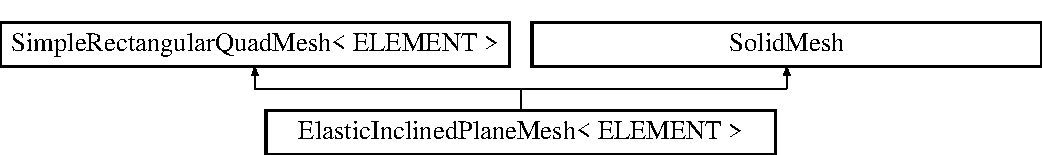
\includegraphics[height=2.000000cm]{classElasticInclinedPlaneMesh}
\end{center}
\end{figure}
\subsection*{Public Member Functions}
\begin{DoxyCompactItemize}
\item 
\hyperlink{classElasticInclinedPlaneMesh_a61ba6d852505dd1353e791223fdfce04}{Elastic\+Inclined\+Plane\+Mesh} (const unsigned \&nx, const unsigned \&ny, const double \&lx, const double \&ly, Time\+Stepper $\ast$time\+\_\+stepper\+\_\+pt)
\end{DoxyCompactItemize}


\subsection{Detailed Description}
\subsubsection*{template$<$class E\+L\+E\+M\+E\+NT$>$\newline
class Elastic\+Inclined\+Plane\+Mesh$<$ E\+L\+E\+M\+E\+N\+T $>$}

Create an Elastic mesh for the problem. 

Definition at line 668 of file inclined\+\_\+plane.\+cc.



\subsection{Constructor \& Destructor Documentation}
\mbox{\Hypertarget{classElasticInclinedPlaneMesh_a61ba6d852505dd1353e791223fdfce04}\label{classElasticInclinedPlaneMesh_a61ba6d852505dd1353e791223fdfce04}} 
\index{Elastic\+Inclined\+Plane\+Mesh@{Elastic\+Inclined\+Plane\+Mesh}!Elastic\+Inclined\+Plane\+Mesh@{Elastic\+Inclined\+Plane\+Mesh}}
\index{Elastic\+Inclined\+Plane\+Mesh@{Elastic\+Inclined\+Plane\+Mesh}!Elastic\+Inclined\+Plane\+Mesh@{Elastic\+Inclined\+Plane\+Mesh}}
\subsubsection{\texorpdfstring{Elastic\+Inclined\+Plane\+Mesh()}{ElasticInclinedPlaneMesh()}}
{\footnotesize\ttfamily template$<$class E\+L\+E\+M\+E\+NT$>$ \\
\hyperlink{classElasticInclinedPlaneMesh}{Elastic\+Inclined\+Plane\+Mesh}$<$ E\+L\+E\+M\+E\+NT $>$\+::\hyperlink{classElasticInclinedPlaneMesh}{Elastic\+Inclined\+Plane\+Mesh} (\begin{DoxyParamCaption}\item[{const unsigned \&}]{nx,  }\item[{const unsigned \&}]{ny,  }\item[{const double \&}]{lx,  }\item[{const double \&}]{ly,  }\item[{Time\+Stepper $\ast$}]{time\+\_\+stepper\+\_\+pt }\end{DoxyParamCaption})\hspace{0.3cm}{\ttfamily [inline]}}



Definition at line 674 of file inclined\+\_\+plane.\+cc.



The documentation for this class was generated from the following file\+:\begin{DoxyCompactItemize}
\item 
\hyperlink{inclined__plane_8cc}{inclined\+\_\+plane.\+cc}\end{DoxyCompactItemize}

\hypertarget{classElasticInclinedPlaneProblem}{}\section{Elastic\+Inclined\+Plane\+Problem$<$ E\+L\+E\+M\+E\+NT, T\+I\+M\+E\+S\+T\+E\+P\+P\+ER $>$ Class Template Reference}
\label{classElasticInclinedPlaneProblem}\index{Elastic\+Inclined\+Plane\+Problem$<$ E\+L\+E\+M\+E\+N\+T, T\+I\+M\+E\+S\+T\+E\+P\+P\+E\+R $>$@{Elastic\+Inclined\+Plane\+Problem$<$ E\+L\+E\+M\+E\+N\+T, T\+I\+M\+E\+S\+T\+E\+P\+P\+E\+R $>$}}
Inheritance diagram for Elastic\+Inclined\+Plane\+Problem$<$ E\+L\+E\+M\+E\+NT, T\+I\+M\+E\+S\+T\+E\+P\+P\+ER $>$\+:\begin{figure}[H]
\begin{center}
\leavevmode
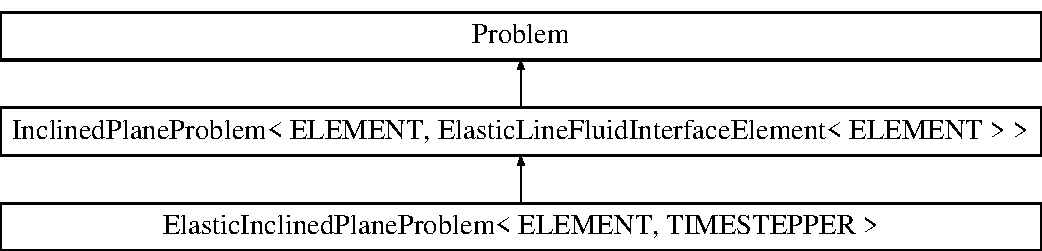
\includegraphics[height=3.000000cm]{classElasticInclinedPlaneProblem}
\end{center}
\end{figure}
\subsection*{Public Member Functions}
\begin{DoxyCompactItemize}
\item 
\hyperlink{classElasticInclinedPlaneProblem_a5006b73d91fcb4bd20d0591577e50f61}{Elastic\+Inclined\+Plane\+Problem} (const unsigned \&nx, const unsigned \&ny, const double \&length)
\item 
void \hyperlink{classElasticInclinedPlaneProblem_a7e61d0cb5e10b7e98f949a43749477a6}{actions\+\_\+after\+\_\+implicit\+\_\+timestep} ()
\begin{DoxyCompactList}\small\item\em Update Lagrangian positions after each timestep (updated-\/lagrangian approach) \end{DoxyCompactList}\end{DoxyCompactItemize}
\subsection*{Additional Inherited Members}


\subsection{Detailed Description}
\subsubsection*{template$<$class E\+L\+E\+M\+E\+NT, class T\+I\+M\+E\+S\+T\+E\+P\+P\+ER$>$\newline
class Elastic\+Inclined\+Plane\+Problem$<$ E\+L\+E\+M\+E\+N\+T, T\+I\+M\+E\+S\+T\+E\+P\+P\+E\+R $>$}



Definition at line 691 of file inclined\+\_\+plane.\+cc.



\subsection{Constructor \& Destructor Documentation}
\mbox{\Hypertarget{classElasticInclinedPlaneProblem_a5006b73d91fcb4bd20d0591577e50f61}\label{classElasticInclinedPlaneProblem_a5006b73d91fcb4bd20d0591577e50f61}} 
\index{Elastic\+Inclined\+Plane\+Problem@{Elastic\+Inclined\+Plane\+Problem}!Elastic\+Inclined\+Plane\+Problem@{Elastic\+Inclined\+Plane\+Problem}}
\index{Elastic\+Inclined\+Plane\+Problem@{Elastic\+Inclined\+Plane\+Problem}!Elastic\+Inclined\+Plane\+Problem@{Elastic\+Inclined\+Plane\+Problem}}
\subsubsection{\texorpdfstring{Elastic\+Inclined\+Plane\+Problem()}{ElasticInclinedPlaneProblem()}}
{\footnotesize\ttfamily template$<$class E\+L\+E\+M\+E\+NT , class T\+I\+M\+E\+S\+T\+E\+P\+P\+ER $>$ \\
\hyperlink{classElasticInclinedPlaneProblem}{Elastic\+Inclined\+Plane\+Problem}$<$ E\+L\+E\+M\+E\+NT, T\+I\+M\+E\+S\+T\+E\+P\+P\+ER $>$\+::\hyperlink{classElasticInclinedPlaneProblem}{Elastic\+Inclined\+Plane\+Problem} (\begin{DoxyParamCaption}\item[{const unsigned \&}]{nx,  }\item[{const unsigned \&}]{ny,  }\item[{const double \&}]{length }\end{DoxyParamCaption})\hspace{0.3cm}{\ttfamily [inline]}}



Definition at line 696 of file inclined\+\_\+plane.\+cc.



References Global\+\_\+\+Physical\+\_\+\+Variables\+::\+Constitutive\+\_\+law\+\_\+pt.



\subsection{Member Function Documentation}
\mbox{\Hypertarget{classElasticInclinedPlaneProblem_a7e61d0cb5e10b7e98f949a43749477a6}\label{classElasticInclinedPlaneProblem_a7e61d0cb5e10b7e98f949a43749477a6}} 
\index{Elastic\+Inclined\+Plane\+Problem@{Elastic\+Inclined\+Plane\+Problem}!actions\+\_\+after\+\_\+implicit\+\_\+timestep@{actions\+\_\+after\+\_\+implicit\+\_\+timestep}}
\index{actions\+\_\+after\+\_\+implicit\+\_\+timestep@{actions\+\_\+after\+\_\+implicit\+\_\+timestep}!Elastic\+Inclined\+Plane\+Problem@{Elastic\+Inclined\+Plane\+Problem}}
\subsubsection{\texorpdfstring{actions\+\_\+after\+\_\+implicit\+\_\+timestep()}{actions\_after\_implicit\_timestep()}}
{\footnotesize\ttfamily template$<$class E\+L\+E\+M\+E\+NT , class T\+I\+M\+E\+S\+T\+E\+P\+P\+ER $>$ \\
void \hyperlink{classElasticInclinedPlaneProblem}{Elastic\+Inclined\+Plane\+Problem}$<$ E\+L\+E\+M\+E\+NT, T\+I\+M\+E\+S\+T\+E\+P\+P\+ER $>$\+::actions\+\_\+after\+\_\+implicit\+\_\+timestep (\begin{DoxyParamCaption}{ }\end{DoxyParamCaption})\hspace{0.3cm}{\ttfamily [inline]}}



Update Lagrangian positions after each timestep (updated-\/lagrangian approach) 



Definition at line 743 of file inclined\+\_\+plane.\+cc.



The documentation for this class was generated from the following file\+:\begin{DoxyCompactItemize}
\item 
\hyperlink{inclined__plane_8cc}{inclined\+\_\+plane.\+cc}\end{DoxyCompactItemize}

\hypertarget{classInclinedPlaneProblem}{}\section{Inclined\+Plane\+Problem$<$ E\+L\+E\+M\+E\+NT, I\+N\+T\+E\+R\+F\+A\+C\+E\+\_\+\+E\+L\+E\+M\+E\+NT $>$ Class Template Reference}
\label{classInclinedPlaneProblem}\index{Inclined\+Plane\+Problem$<$ E\+L\+E\+M\+E\+N\+T, I\+N\+T\+E\+R\+F\+A\+C\+E\+\_\+\+E\+L\+E\+M\+E\+N\+T $>$@{Inclined\+Plane\+Problem$<$ E\+L\+E\+M\+E\+N\+T, I\+N\+T\+E\+R\+F\+A\+C\+E\+\_\+\+E\+L\+E\+M\+E\+N\+T $>$}}


Generic problem class that will form the base class for both spine and elastic mesh-\/updates of the problem. Templated by the bulk element and interface element types.  


Inheritance diagram for Inclined\+Plane\+Problem$<$ E\+L\+E\+M\+E\+NT, I\+N\+T\+E\+R\+F\+A\+C\+E\+\_\+\+E\+L\+E\+M\+E\+NT $>$\+:\begin{figure}[H]
\begin{center}
\leavevmode
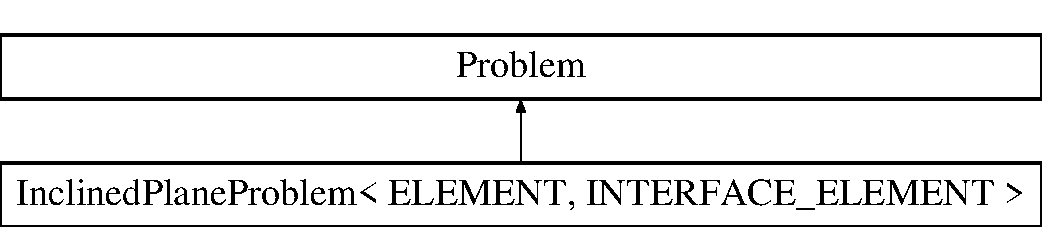
\includegraphics[height=2.000000cm]{classInclinedPlaneProblem}
\end{center}
\end{figure}
\subsection*{Public Member Functions}
\begin{DoxyCompactItemize}
\item 
\hyperlink{classInclinedPlaneProblem_a52d15d242c8f17a340914996b49a32a3}{Inclined\+Plane\+Problem} (const unsigned \&nx, const unsigned \&ny, const double \&length)
\begin{DoxyCompactList}\small\item\em Generic Constructor (empty) \end{DoxyCompactList}\item 
void \hyperlink{classInclinedPlaneProblem_a0e2fcfdb8230df82729ba7d728e58040}{solve\+\_\+steady} ()
\begin{DoxyCompactList}\small\item\em Solve the steady problem. \end{DoxyCompactList}\item 
void \hyperlink{classInclinedPlaneProblem_a74bbd1ccfd3dd82c999a16924c230f51}{timestep} (const double \&dt, const unsigned \&n\+\_\+tsteps)
\begin{DoxyCompactList}\small\item\em Take n\+\_\+tsteps timesteps of size dt. \end{DoxyCompactList}\item 
void \hyperlink{classInclinedPlaneProblem_af9cf7a9677e823c52f1646105dfa7937}{actions\+\_\+before\+\_\+implicit\+\_\+timestep} ()
\begin{DoxyCompactList}\small\item\em Actions before the timestep (update the time-\/dependent boundary conditions) \end{DoxyCompactList}\item 
void \hyperlink{classInclinedPlaneProblem_a39ab8005f7603bd1f06f13d6e7a3ae64}{make\+\_\+traction\+\_\+elements} ()
\begin{DoxyCompactList}\small\item\em Function to add the traction boundary elements to boundaries 3(inlet) and 1(outlet) of the mesh. \end{DoxyCompactList}\item 
void \hyperlink{classInclinedPlaneProblem_a78d06d406af81a3dddbec0a31b65e8a4}{make\+\_\+free\+\_\+surface\+\_\+elements} ()
\item 
void \hyperlink{classInclinedPlaneProblem_ae44e360be4a46e1343c3960c3a43380f}{complete\+\_\+build} ()
\begin{DoxyCompactList}\small\item\em Complete the build of the problem setting all standard parameters and boundary conditions. \end{DoxyCompactList}\item 
\hyperlink{classInclinedPlaneProblem_ad89c7dc7975bf128a7c249496fabc97f}{$\sim$\+Inclined\+Plane\+Problem} ()
\begin{DoxyCompactList}\small\item\em Generic desructor to clean up the memory allocated in the problem. \end{DoxyCompactList}\end{DoxyCompactItemize}
\subsection*{Protected Attributes}
\begin{DoxyCompactItemize}
\item 
Mesh $\ast$ \hyperlink{classInclinedPlaneProblem_a20c506fe684dc146424b8ec019239783}{Bulk\+\_\+mesh\+\_\+pt}
\begin{DoxyCompactList}\small\item\em Bulk fluid mesh. \end{DoxyCompactList}\item 
Mesh $\ast$ \hyperlink{classInclinedPlaneProblem_a85bcc36a8ad4ad7aa3595585e73a3197}{Traction\+\_\+mesh\+\_\+pt}
\begin{DoxyCompactList}\small\item\em Mesh for the traction elements that are added at inlet and outlet. \end{DoxyCompactList}\item 
Mesh $\ast$ \hyperlink{classInclinedPlaneProblem_aba36d367278218bf00356c3bee0733a0}{Surface\+\_\+mesh\+\_\+pt}
\begin{DoxyCompactList}\small\item\em Mesh for the free surface elements. \end{DoxyCompactList}\item 
Mesh $\ast$ \hyperlink{classInclinedPlaneProblem_adefbac5880323d7de622e2ba0c526746}{Point\+\_\+mesh\+\_\+pt}
\begin{DoxyCompactList}\small\item\em Mesh for the point elements at each end of the free surface. \end{DoxyCompactList}\item 
std\+::string \hyperlink{classInclinedPlaneProblem_a6ad45c76bd24f63c0162313042ce2e7d}{Output\+\_\+prefix}
\begin{DoxyCompactList}\small\item\em Prefix for output files. \end{DoxyCompactList}\end{DoxyCompactItemize}


\subsection{Detailed Description}
\subsubsection*{template$<$class E\+L\+E\+M\+E\+NT, class I\+N\+T\+E\+R\+F\+A\+C\+E\+\_\+\+E\+L\+E\+M\+E\+NT$>$\newline
class Inclined\+Plane\+Problem$<$ E\+L\+E\+M\+E\+N\+T, I\+N\+T\+E\+R\+F\+A\+C\+E\+\_\+\+E\+L\+E\+M\+E\+N\+T $>$}

Generic problem class that will form the base class for both spine and elastic mesh-\/updates of the problem. Templated by the bulk element and interface element types. 

Definition at line 142 of file inclined\+\_\+plane.\+cc.



\subsection{Constructor \& Destructor Documentation}
\mbox{\Hypertarget{classInclinedPlaneProblem_a52d15d242c8f17a340914996b49a32a3}\label{classInclinedPlaneProblem_a52d15d242c8f17a340914996b49a32a3}} 
\index{Inclined\+Plane\+Problem@{Inclined\+Plane\+Problem}!Inclined\+Plane\+Problem@{Inclined\+Plane\+Problem}}
\index{Inclined\+Plane\+Problem@{Inclined\+Plane\+Problem}!Inclined\+Plane\+Problem@{Inclined\+Plane\+Problem}}
\subsubsection{\texorpdfstring{Inclined\+Plane\+Problem()}{InclinedPlaneProblem()}}
{\footnotesize\ttfamily template$<$class E\+L\+E\+M\+E\+NT, class I\+N\+T\+E\+R\+F\+A\+C\+E\+\_\+\+E\+L\+E\+M\+E\+NT$>$ \\
\hyperlink{classInclinedPlaneProblem}{Inclined\+Plane\+Problem}$<$ E\+L\+E\+M\+E\+NT, I\+N\+T\+E\+R\+F\+A\+C\+E\+\_\+\+E\+L\+E\+M\+E\+NT $>$\+::\hyperlink{classInclinedPlaneProblem}{Inclined\+Plane\+Problem} (\begin{DoxyParamCaption}\item[{const unsigned \&}]{nx,  }\item[{const unsigned \&}]{ny,  }\item[{const double \&}]{length }\end{DoxyParamCaption})\hspace{0.3cm}{\ttfamily [inline]}}



Generic Constructor (empty) 



Definition at line 165 of file inclined\+\_\+plane.\+cc.

\mbox{\Hypertarget{classInclinedPlaneProblem_ad89c7dc7975bf128a7c249496fabc97f}\label{classInclinedPlaneProblem_ad89c7dc7975bf128a7c249496fabc97f}} 
\index{Inclined\+Plane\+Problem@{Inclined\+Plane\+Problem}!````~Inclined\+Plane\+Problem@{$\sim$\+Inclined\+Plane\+Problem}}
\index{````~Inclined\+Plane\+Problem@{$\sim$\+Inclined\+Plane\+Problem}!Inclined\+Plane\+Problem@{Inclined\+Plane\+Problem}}
\subsubsection{\texorpdfstring{$\sim$\+Inclined\+Plane\+Problem()}{~InclinedPlaneProblem()}}
{\footnotesize\ttfamily template$<$class E\+L\+E\+M\+E\+NT, class I\+N\+T\+E\+R\+F\+A\+C\+E\+\_\+\+E\+L\+E\+M\+E\+NT$>$ \\
\hyperlink{classInclinedPlaneProblem}{Inclined\+Plane\+Problem}$<$ E\+L\+E\+M\+E\+NT, I\+N\+T\+E\+R\+F\+A\+C\+E\+\_\+\+E\+L\+E\+M\+E\+NT $>$\+::$\sim$\hyperlink{classInclinedPlaneProblem}{Inclined\+Plane\+Problem} (\begin{DoxyParamCaption}{ }\end{DoxyParamCaption})\hspace{0.3cm}{\ttfamily [inline]}}



Generic desructor to clean up the memory allocated in the problem. 



Definition at line 389 of file inclined\+\_\+plane.\+cc.



\subsection{Member Function Documentation}
\mbox{\Hypertarget{classInclinedPlaneProblem_af9cf7a9677e823c52f1646105dfa7937}\label{classInclinedPlaneProblem_af9cf7a9677e823c52f1646105dfa7937}} 
\index{Inclined\+Plane\+Problem@{Inclined\+Plane\+Problem}!actions\+\_\+before\+\_\+implicit\+\_\+timestep@{actions\+\_\+before\+\_\+implicit\+\_\+timestep}}
\index{actions\+\_\+before\+\_\+implicit\+\_\+timestep@{actions\+\_\+before\+\_\+implicit\+\_\+timestep}!Inclined\+Plane\+Problem@{Inclined\+Plane\+Problem}}
\subsubsection{\texorpdfstring{actions\+\_\+before\+\_\+implicit\+\_\+timestep()}{actions\_before\_implicit\_timestep()}}
{\footnotesize\ttfamily template$<$class E\+L\+E\+M\+E\+NT, class I\+N\+T\+E\+R\+F\+A\+C\+E\+\_\+\+E\+L\+E\+M\+E\+NT$>$ \\
void \hyperlink{classInclinedPlaneProblem}{Inclined\+Plane\+Problem}$<$ E\+L\+E\+M\+E\+NT, I\+N\+T\+E\+R\+F\+A\+C\+E\+\_\+\+E\+L\+E\+M\+E\+NT $>$\+::actions\+\_\+before\+\_\+implicit\+\_\+timestep (\begin{DoxyParamCaption}{ }\end{DoxyParamCaption})\hspace{0.3cm}{\ttfamily [inline]}}



Actions before the timestep (update the time-\/dependent boundary conditions) 



Definition at line 177 of file inclined\+\_\+plane.\+cc.

\mbox{\Hypertarget{classInclinedPlaneProblem_ae44e360be4a46e1343c3960c3a43380f}\label{classInclinedPlaneProblem_ae44e360be4a46e1343c3960c3a43380f}} 
\index{Inclined\+Plane\+Problem@{Inclined\+Plane\+Problem}!complete\+\_\+build@{complete\+\_\+build}}
\index{complete\+\_\+build@{complete\+\_\+build}!Inclined\+Plane\+Problem@{Inclined\+Plane\+Problem}}
\subsubsection{\texorpdfstring{complete\+\_\+build()}{complete\_build()}}
{\footnotesize\ttfamily template$<$class E\+L\+E\+M\+E\+NT, class I\+N\+T\+E\+R\+F\+A\+C\+E\+\_\+\+E\+L\+E\+M\+E\+NT$>$ \\
void \hyperlink{classInclinedPlaneProblem}{Inclined\+Plane\+Problem}$<$ E\+L\+E\+M\+E\+NT, I\+N\+T\+E\+R\+F\+A\+C\+E\+\_\+\+E\+L\+E\+M\+E\+NT $>$\+::complete\+\_\+build (\begin{DoxyParamCaption}{ }\end{DoxyParamCaption})\hspace{0.3cm}{\ttfamily [inline]}}



Complete the build of the problem setting all standard parameters and boundary conditions. 



Definition at line 304 of file inclined\+\_\+plane.\+cc.

\mbox{\Hypertarget{classInclinedPlaneProblem_a78d06d406af81a3dddbec0a31b65e8a4}\label{classInclinedPlaneProblem_a78d06d406af81a3dddbec0a31b65e8a4}} 
\index{Inclined\+Plane\+Problem@{Inclined\+Plane\+Problem}!make\+\_\+free\+\_\+surface\+\_\+elements@{make\+\_\+free\+\_\+surface\+\_\+elements}}
\index{make\+\_\+free\+\_\+surface\+\_\+elements@{make\+\_\+free\+\_\+surface\+\_\+elements}!Inclined\+Plane\+Problem@{Inclined\+Plane\+Problem}}
\subsubsection{\texorpdfstring{make\+\_\+free\+\_\+surface\+\_\+elements()}{make\_free\_surface\_elements()}}
{\footnotesize\ttfamily template$<$class E\+L\+E\+M\+E\+NT, class I\+N\+T\+E\+R\+F\+A\+C\+E\+\_\+\+E\+L\+E\+M\+E\+NT$>$ \\
void \hyperlink{classInclinedPlaneProblem}{Inclined\+Plane\+Problem}$<$ E\+L\+E\+M\+E\+NT, I\+N\+T\+E\+R\+F\+A\+C\+E\+\_\+\+E\+L\+E\+M\+E\+NT $>$\+::make\+\_\+free\+\_\+surface\+\_\+elements (\begin{DoxyParamCaption}{ }\end{DoxyParamCaption})\hspace{0.3cm}{\ttfamily [inline]}}



Definition at line 243 of file inclined\+\_\+plane.\+cc.

\mbox{\Hypertarget{classInclinedPlaneProblem_a39ab8005f7603bd1f06f13d6e7a3ae64}\label{classInclinedPlaneProblem_a39ab8005f7603bd1f06f13d6e7a3ae64}} 
\index{Inclined\+Plane\+Problem@{Inclined\+Plane\+Problem}!make\+\_\+traction\+\_\+elements@{make\+\_\+traction\+\_\+elements}}
\index{make\+\_\+traction\+\_\+elements@{make\+\_\+traction\+\_\+elements}!Inclined\+Plane\+Problem@{Inclined\+Plane\+Problem}}
\subsubsection{\texorpdfstring{make\+\_\+traction\+\_\+elements()}{make\_traction\_elements()}}
{\footnotesize\ttfamily template$<$class E\+L\+E\+M\+E\+NT, class I\+N\+T\+E\+R\+F\+A\+C\+E\+\_\+\+E\+L\+E\+M\+E\+NT$>$ \\
void \hyperlink{classInclinedPlaneProblem}{Inclined\+Plane\+Problem}$<$ E\+L\+E\+M\+E\+NT, I\+N\+T\+E\+R\+F\+A\+C\+E\+\_\+\+E\+L\+E\+M\+E\+NT $>$\+::make\+\_\+traction\+\_\+elements (\begin{DoxyParamCaption}{ }\end{DoxyParamCaption})\hspace{0.3cm}{\ttfamily [inline]}}



Function to add the traction boundary elements to boundaries 3(inlet) and 1(outlet) of the mesh. 



Definition at line 197 of file inclined\+\_\+plane.\+cc.

\mbox{\Hypertarget{classInclinedPlaneProblem_a0e2fcfdb8230df82729ba7d728e58040}\label{classInclinedPlaneProblem_a0e2fcfdb8230df82729ba7d728e58040}} 
\index{Inclined\+Plane\+Problem@{Inclined\+Plane\+Problem}!solve\+\_\+steady@{solve\+\_\+steady}}
\index{solve\+\_\+steady@{solve\+\_\+steady}!Inclined\+Plane\+Problem@{Inclined\+Plane\+Problem}}
\subsubsection{\texorpdfstring{solve\+\_\+steady()}{solve\_steady()}}
{\footnotesize\ttfamily template$<$class E\+L\+E\+M\+E\+NT , class I\+N\+T\+E\+R\+F\+A\+C\+E\+\_\+\+E\+L\+E\+M\+E\+NT $>$ \\
void \hyperlink{classInclinedPlaneProblem}{Inclined\+Plane\+Problem}$<$ E\+L\+E\+M\+E\+NT, I\+N\+T\+E\+R\+F\+A\+C\+E\+\_\+\+E\+L\+E\+M\+E\+NT $>$\+::solve\+\_\+steady (\begin{DoxyParamCaption}{ }\end{DoxyParamCaption})}



Solve the steady problem. 



Definition at line 415 of file inclined\+\_\+plane.\+cc.

\mbox{\Hypertarget{classInclinedPlaneProblem_a74bbd1ccfd3dd82c999a16924c230f51}\label{classInclinedPlaneProblem_a74bbd1ccfd3dd82c999a16924c230f51}} 
\index{Inclined\+Plane\+Problem@{Inclined\+Plane\+Problem}!timestep@{timestep}}
\index{timestep@{timestep}!Inclined\+Plane\+Problem@{Inclined\+Plane\+Problem}}
\subsubsection{\texorpdfstring{timestep()}{timestep()}}
{\footnotesize\ttfamily template$<$class E\+L\+E\+M\+E\+NT , class I\+N\+T\+E\+R\+F\+A\+C\+E\+\_\+\+E\+L\+E\+M\+E\+NT $>$ \\
void \hyperlink{classInclinedPlaneProblem}{Inclined\+Plane\+Problem}$<$ E\+L\+E\+M\+E\+NT, I\+N\+T\+E\+R\+F\+A\+C\+E\+\_\+\+E\+L\+E\+M\+E\+NT $>$\+::timestep (\begin{DoxyParamCaption}\item[{const double \&}]{dt,  }\item[{const unsigned \&}]{n\+\_\+tsteps }\end{DoxyParamCaption})}



Take n\+\_\+tsteps timesteps of size dt. 

Perform n\+\_\+tsteps timesteps of size dt. 

Definition at line 448 of file inclined\+\_\+plane.\+cc.



Referenced by Inclined\+Plane\+Problem$<$ E\+L\+E\+M\+E\+N\+T, Elastic\+Line\+Fluid\+Interface\+Element$<$ E\+L\+E\+M\+E\+N\+T $>$ $>$\+::solve\+\_\+steady().



\subsection{Member Data Documentation}
\mbox{\Hypertarget{classInclinedPlaneProblem_a20c506fe684dc146424b8ec019239783}\label{classInclinedPlaneProblem_a20c506fe684dc146424b8ec019239783}} 
\index{Inclined\+Plane\+Problem@{Inclined\+Plane\+Problem}!Bulk\+\_\+mesh\+\_\+pt@{Bulk\+\_\+mesh\+\_\+pt}}
\index{Bulk\+\_\+mesh\+\_\+pt@{Bulk\+\_\+mesh\+\_\+pt}!Inclined\+Plane\+Problem@{Inclined\+Plane\+Problem}}
\subsubsection{\texorpdfstring{Bulk\+\_\+mesh\+\_\+pt}{Bulk\_mesh\_pt}}
{\footnotesize\ttfamily template$<$class E\+L\+E\+M\+E\+NT, class I\+N\+T\+E\+R\+F\+A\+C\+E\+\_\+\+E\+L\+E\+M\+E\+NT$>$ \\
Mesh$\ast$ \hyperlink{classInclinedPlaneProblem}{Inclined\+Plane\+Problem}$<$ E\+L\+E\+M\+E\+NT, I\+N\+T\+E\+R\+F\+A\+C\+E\+\_\+\+E\+L\+E\+M\+E\+NT $>$\+::Bulk\+\_\+mesh\+\_\+pt\hspace{0.3cm}{\ttfamily [protected]}}



Bulk fluid mesh. 



Definition at line 148 of file inclined\+\_\+plane.\+cc.

\mbox{\Hypertarget{classInclinedPlaneProblem_a6ad45c76bd24f63c0162313042ce2e7d}\label{classInclinedPlaneProblem_a6ad45c76bd24f63c0162313042ce2e7d}} 
\index{Inclined\+Plane\+Problem@{Inclined\+Plane\+Problem}!Output\+\_\+prefix@{Output\+\_\+prefix}}
\index{Output\+\_\+prefix@{Output\+\_\+prefix}!Inclined\+Plane\+Problem@{Inclined\+Plane\+Problem}}
\subsubsection{\texorpdfstring{Output\+\_\+prefix}{Output\_prefix}}
{\footnotesize\ttfamily template$<$class E\+L\+E\+M\+E\+NT, class I\+N\+T\+E\+R\+F\+A\+C\+E\+\_\+\+E\+L\+E\+M\+E\+NT$>$ \\
std\+::string \hyperlink{classInclinedPlaneProblem}{Inclined\+Plane\+Problem}$<$ E\+L\+E\+M\+E\+NT, I\+N\+T\+E\+R\+F\+A\+C\+E\+\_\+\+E\+L\+E\+M\+E\+NT $>$\+::Output\+\_\+prefix\hspace{0.3cm}{\ttfamily [protected]}}



Prefix for output files. 



Definition at line 160 of file inclined\+\_\+plane.\+cc.

\mbox{\Hypertarget{classInclinedPlaneProblem_adefbac5880323d7de622e2ba0c526746}\label{classInclinedPlaneProblem_adefbac5880323d7de622e2ba0c526746}} 
\index{Inclined\+Plane\+Problem@{Inclined\+Plane\+Problem}!Point\+\_\+mesh\+\_\+pt@{Point\+\_\+mesh\+\_\+pt}}
\index{Point\+\_\+mesh\+\_\+pt@{Point\+\_\+mesh\+\_\+pt}!Inclined\+Plane\+Problem@{Inclined\+Plane\+Problem}}
\subsubsection{\texorpdfstring{Point\+\_\+mesh\+\_\+pt}{Point\_mesh\_pt}}
{\footnotesize\ttfamily template$<$class E\+L\+E\+M\+E\+NT, class I\+N\+T\+E\+R\+F\+A\+C\+E\+\_\+\+E\+L\+E\+M\+E\+NT$>$ \\
Mesh$\ast$ \hyperlink{classInclinedPlaneProblem}{Inclined\+Plane\+Problem}$<$ E\+L\+E\+M\+E\+NT, I\+N\+T\+E\+R\+F\+A\+C\+E\+\_\+\+E\+L\+E\+M\+E\+NT $>$\+::Point\+\_\+mesh\+\_\+pt\hspace{0.3cm}{\ttfamily [protected]}}



Mesh for the point elements at each end of the free surface. 



Definition at line 157 of file inclined\+\_\+plane.\+cc.

\mbox{\Hypertarget{classInclinedPlaneProblem_aba36d367278218bf00356c3bee0733a0}\label{classInclinedPlaneProblem_aba36d367278218bf00356c3bee0733a0}} 
\index{Inclined\+Plane\+Problem@{Inclined\+Plane\+Problem}!Surface\+\_\+mesh\+\_\+pt@{Surface\+\_\+mesh\+\_\+pt}}
\index{Surface\+\_\+mesh\+\_\+pt@{Surface\+\_\+mesh\+\_\+pt}!Inclined\+Plane\+Problem@{Inclined\+Plane\+Problem}}
\subsubsection{\texorpdfstring{Surface\+\_\+mesh\+\_\+pt}{Surface\_mesh\_pt}}
{\footnotesize\ttfamily template$<$class E\+L\+E\+M\+E\+NT, class I\+N\+T\+E\+R\+F\+A\+C\+E\+\_\+\+E\+L\+E\+M\+E\+NT$>$ \\
Mesh$\ast$ \hyperlink{classInclinedPlaneProblem}{Inclined\+Plane\+Problem}$<$ E\+L\+E\+M\+E\+NT, I\+N\+T\+E\+R\+F\+A\+C\+E\+\_\+\+E\+L\+E\+M\+E\+NT $>$\+::Surface\+\_\+mesh\+\_\+pt\hspace{0.3cm}{\ttfamily [protected]}}



Mesh for the free surface elements. 



Definition at line 154 of file inclined\+\_\+plane.\+cc.

\mbox{\Hypertarget{classInclinedPlaneProblem_a85bcc36a8ad4ad7aa3595585e73a3197}\label{classInclinedPlaneProblem_a85bcc36a8ad4ad7aa3595585e73a3197}} 
\index{Inclined\+Plane\+Problem@{Inclined\+Plane\+Problem}!Traction\+\_\+mesh\+\_\+pt@{Traction\+\_\+mesh\+\_\+pt}}
\index{Traction\+\_\+mesh\+\_\+pt@{Traction\+\_\+mesh\+\_\+pt}!Inclined\+Plane\+Problem@{Inclined\+Plane\+Problem}}
\subsubsection{\texorpdfstring{Traction\+\_\+mesh\+\_\+pt}{Traction\_mesh\_pt}}
{\footnotesize\ttfamily template$<$class E\+L\+E\+M\+E\+NT, class I\+N\+T\+E\+R\+F\+A\+C\+E\+\_\+\+E\+L\+E\+M\+E\+NT$>$ \\
Mesh$\ast$ \hyperlink{classInclinedPlaneProblem}{Inclined\+Plane\+Problem}$<$ E\+L\+E\+M\+E\+NT, I\+N\+T\+E\+R\+F\+A\+C\+E\+\_\+\+E\+L\+E\+M\+E\+NT $>$\+::Traction\+\_\+mesh\+\_\+pt\hspace{0.3cm}{\ttfamily [protected]}}



Mesh for the traction elements that are added at inlet and outlet. 



Definition at line 151 of file inclined\+\_\+plane.\+cc.



The documentation for this class was generated from the following file\+:\begin{DoxyCompactItemize}
\item 
\hyperlink{inclined__plane_8cc}{inclined\+\_\+plane.\+cc}\end{DoxyCompactItemize}

\hypertarget{classSpineInclinedPlaneMesh}{}\section{Spine\+Inclined\+Plane\+Mesh$<$ E\+L\+E\+M\+E\+NT $>$ Class Template Reference}
\label{classSpineInclinedPlaneMesh}\index{Spine\+Inclined\+Plane\+Mesh$<$ E\+L\+E\+M\+E\+N\+T $>$@{Spine\+Inclined\+Plane\+Mesh$<$ E\+L\+E\+M\+E\+N\+T $>$}}


Create a spine mesh for the problem.  


Inheritance diagram for Spine\+Inclined\+Plane\+Mesh$<$ E\+L\+E\+M\+E\+NT $>$\+:\begin{figure}[H]
\begin{center}
\leavevmode
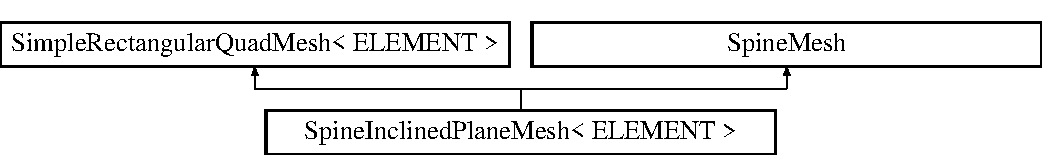
\includegraphics[height=2.000000cm]{classSpineInclinedPlaneMesh}
\end{center}
\end{figure}
\subsection*{Public Member Functions}
\begin{DoxyCompactItemize}
\item 
\hyperlink{classSpineInclinedPlaneMesh_a97e770220d4cd41e11c86c5cfa289133}{Spine\+Inclined\+Plane\+Mesh} (const unsigned \&nx, const unsigned \&ny, const double \&lx, const double \&ly, Time\+Stepper $\ast$time\+\_\+stepper\+\_\+pt)
\item 
virtual void \hyperlink{classSpineInclinedPlaneMesh_a01fa9c443029a6a00b1679a6785029f6}{spine\+\_\+node\+\_\+update} (Spine\+Node $\ast$spine\+\_\+node\+\_\+pt)
\begin{DoxyCompactList}\small\item\em General node update function implements pure virtual function defined in Spine\+Mesh base class and performs specific node update actions\+: along vertical spines. \end{DoxyCompactList}\end{DoxyCompactItemize}


\subsection{Detailed Description}
\subsubsection*{template$<$class E\+L\+E\+M\+E\+NT$>$\newline
class Spine\+Inclined\+Plane\+Mesh$<$ E\+L\+E\+M\+E\+N\+T $>$}

Create a spine mesh for the problem. 

Definition at line 526 of file inclined\+\_\+plane.\+cc.



\subsection{Constructor \& Destructor Documentation}
\mbox{\Hypertarget{classSpineInclinedPlaneMesh_a97e770220d4cd41e11c86c5cfa289133}\label{classSpineInclinedPlaneMesh_a97e770220d4cd41e11c86c5cfa289133}} 
\index{Spine\+Inclined\+Plane\+Mesh@{Spine\+Inclined\+Plane\+Mesh}!Spine\+Inclined\+Plane\+Mesh@{Spine\+Inclined\+Plane\+Mesh}}
\index{Spine\+Inclined\+Plane\+Mesh@{Spine\+Inclined\+Plane\+Mesh}!Spine\+Inclined\+Plane\+Mesh@{Spine\+Inclined\+Plane\+Mesh}}
\subsubsection{\texorpdfstring{Spine\+Inclined\+Plane\+Mesh()}{SpineInclinedPlaneMesh()}}
{\footnotesize\ttfamily template$<$class E\+L\+E\+M\+E\+NT$>$ \\
\hyperlink{classSpineInclinedPlaneMesh}{Spine\+Inclined\+Plane\+Mesh}$<$ E\+L\+E\+M\+E\+NT $>$\+::\hyperlink{classSpineInclinedPlaneMesh}{Spine\+Inclined\+Plane\+Mesh} (\begin{DoxyParamCaption}\item[{const unsigned \&}]{nx,  }\item[{const unsigned \&}]{ny,  }\item[{const double \&}]{lx,  }\item[{const double \&}]{ly,  }\item[{Time\+Stepper $\ast$}]{time\+\_\+stepper\+\_\+pt }\end{DoxyParamCaption})\hspace{0.3cm}{\ttfamily [inline]}}



Definition at line 531 of file inclined\+\_\+plane.\+cc.



\subsection{Member Function Documentation}
\mbox{\Hypertarget{classSpineInclinedPlaneMesh_a01fa9c443029a6a00b1679a6785029f6}\label{classSpineInclinedPlaneMesh_a01fa9c443029a6a00b1679a6785029f6}} 
\index{Spine\+Inclined\+Plane\+Mesh@{Spine\+Inclined\+Plane\+Mesh}!spine\+\_\+node\+\_\+update@{spine\+\_\+node\+\_\+update}}
\index{spine\+\_\+node\+\_\+update@{spine\+\_\+node\+\_\+update}!Spine\+Inclined\+Plane\+Mesh@{Spine\+Inclined\+Plane\+Mesh}}
\subsubsection{\texorpdfstring{spine\+\_\+node\+\_\+update()}{spine\_node\_update()}}
{\footnotesize\ttfamily template$<$class E\+L\+E\+M\+E\+NT$>$ \\
virtual void \hyperlink{classSpineInclinedPlaneMesh}{Spine\+Inclined\+Plane\+Mesh}$<$ E\+L\+E\+M\+E\+NT $>$\+::spine\+\_\+node\+\_\+update (\begin{DoxyParamCaption}\item[{Spine\+Node $\ast$}]{spine\+\_\+node\+\_\+pt }\end{DoxyParamCaption})\hspace{0.3cm}{\ttfamily [inline]}, {\ttfamily [virtual]}}



General node update function implements pure virtual function defined in Spine\+Mesh base class and performs specific node update actions\+: along vertical spines. 



Definition at line 594 of file inclined\+\_\+plane.\+cc.



The documentation for this class was generated from the following file\+:\begin{DoxyCompactItemize}
\item 
\hyperlink{inclined__plane_8cc}{inclined\+\_\+plane.\+cc}\end{DoxyCompactItemize}

\hypertarget{classSpineInclinedPlaneProblem}{}\section{Spine\+Inclined\+Plane\+Problem$<$ E\+L\+E\+M\+E\+NT, T\+I\+M\+E\+S\+T\+E\+P\+P\+ER $>$ Class Template Reference}
\label{classSpineInclinedPlaneProblem}\index{Spine\+Inclined\+Plane\+Problem$<$ E\+L\+E\+M\+E\+N\+T, T\+I\+M\+E\+S\+T\+E\+P\+P\+E\+R $>$@{Spine\+Inclined\+Plane\+Problem$<$ E\+L\+E\+M\+E\+N\+T, T\+I\+M\+E\+S\+T\+E\+P\+P\+E\+R $>$}}
Inheritance diagram for Spine\+Inclined\+Plane\+Problem$<$ E\+L\+E\+M\+E\+NT, T\+I\+M\+E\+S\+T\+E\+P\+P\+ER $>$\+:\begin{figure}[H]
\begin{center}
\leavevmode
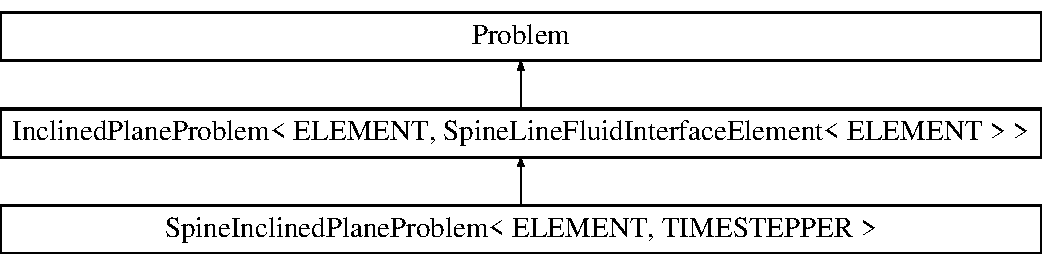
\includegraphics[height=3.000000cm]{classSpineInclinedPlaneProblem}
\end{center}
\end{figure}
\subsection*{Public Member Functions}
\begin{DoxyCompactItemize}
\item 
\hyperlink{classSpineInclinedPlaneProblem_a5eba548aaedf82845fd02403f06a42f7}{Spine\+Inclined\+Plane\+Problem} (const unsigned \&nx, const unsigned \&ny, const double \&length)
\item 
void \hyperlink{classSpineInclinedPlaneProblem_af05f87be8b233df5a296f6375001d385}{actions\+\_\+before\+\_\+newton\+\_\+convergence\+\_\+check} ()
\end{DoxyCompactItemize}
\subsection*{Additional Inherited Members}


\subsection{Detailed Description}
\subsubsection*{template$<$class E\+L\+E\+M\+E\+NT, class T\+I\+M\+E\+S\+T\+E\+P\+P\+ER$>$\newline
class Spine\+Inclined\+Plane\+Problem$<$ E\+L\+E\+M\+E\+N\+T, T\+I\+M\+E\+S\+T\+E\+P\+P\+E\+R $>$}



Definition at line 611 of file inclined\+\_\+plane.\+cc.



\subsection{Constructor \& Destructor Documentation}
\mbox{\Hypertarget{classSpineInclinedPlaneProblem_a5eba548aaedf82845fd02403f06a42f7}\label{classSpineInclinedPlaneProblem_a5eba548aaedf82845fd02403f06a42f7}} 
\index{Spine\+Inclined\+Plane\+Problem@{Spine\+Inclined\+Plane\+Problem}!Spine\+Inclined\+Plane\+Problem@{Spine\+Inclined\+Plane\+Problem}}
\index{Spine\+Inclined\+Plane\+Problem@{Spine\+Inclined\+Plane\+Problem}!Spine\+Inclined\+Plane\+Problem@{Spine\+Inclined\+Plane\+Problem}}
\subsubsection{\texorpdfstring{Spine\+Inclined\+Plane\+Problem()}{SpineInclinedPlaneProblem()}}
{\footnotesize\ttfamily template$<$class E\+L\+E\+M\+E\+NT, class T\+I\+M\+E\+S\+T\+E\+P\+P\+ER$>$ \\
\hyperlink{classSpineInclinedPlaneProblem}{Spine\+Inclined\+Plane\+Problem}$<$ E\+L\+E\+M\+E\+NT, T\+I\+M\+E\+S\+T\+E\+P\+P\+ER $>$\+::\hyperlink{classSpineInclinedPlaneProblem}{Spine\+Inclined\+Plane\+Problem} (\begin{DoxyParamCaption}\item[{const unsigned \&}]{nx,  }\item[{const unsigned \&}]{ny,  }\item[{const double \&}]{length }\end{DoxyParamCaption})\hspace{0.3cm}{\ttfamily [inline]}}



Definition at line 617 of file inclined\+\_\+plane.\+cc.



\subsection{Member Function Documentation}
\mbox{\Hypertarget{classSpineInclinedPlaneProblem_af05f87be8b233df5a296f6375001d385}\label{classSpineInclinedPlaneProblem_af05f87be8b233df5a296f6375001d385}} 
\index{Spine\+Inclined\+Plane\+Problem@{Spine\+Inclined\+Plane\+Problem}!actions\+\_\+before\+\_\+newton\+\_\+convergence\+\_\+check@{actions\+\_\+before\+\_\+newton\+\_\+convergence\+\_\+check}}
\index{actions\+\_\+before\+\_\+newton\+\_\+convergence\+\_\+check@{actions\+\_\+before\+\_\+newton\+\_\+convergence\+\_\+check}!Spine\+Inclined\+Plane\+Problem@{Spine\+Inclined\+Plane\+Problem}}
\subsubsection{\texorpdfstring{actions\+\_\+before\+\_\+newton\+\_\+convergence\+\_\+check()}{actions\_before\_newton\_convergence\_check()}}
{\footnotesize\ttfamily template$<$class E\+L\+E\+M\+E\+NT, class T\+I\+M\+E\+S\+T\+E\+P\+P\+ER$>$ \\
void \hyperlink{classSpineInclinedPlaneProblem}{Spine\+Inclined\+Plane\+Problem}$<$ E\+L\+E\+M\+E\+NT, T\+I\+M\+E\+S\+T\+E\+P\+P\+ER $>$\+::actions\+\_\+before\+\_\+newton\+\_\+convergence\+\_\+check (\begin{DoxyParamCaption}{ }\end{DoxyParamCaption})\hspace{0.3cm}{\ttfamily [inline]}}

Spine heights/lengths are unknowns in the problem so their values get corrected during each Newton step. However, changing their value does not automatically change the nodal positions, so we need to update all of them 

Definition at line 653 of file inclined\+\_\+plane.\+cc.



The documentation for this class was generated from the following file\+:\begin{DoxyCompactItemize}
\item 
\hyperlink{inclined__plane_8cc}{inclined\+\_\+plane.\+cc}\end{DoxyCompactItemize}

\chapter{File Documentation}
\hypertarget{inclined__plane_8cc}{}\section{inclined\+\_\+plane.\+cc File Reference}
\label{inclined__plane_8cc}\index{inclined\+\_\+plane.\+cc@{inclined\+\_\+plane.\+cc}}
\subsection*{Classes}
\begin{DoxyCompactItemize}
\item 
class \hyperlink{classInclinedPlaneProblem}{Inclined\+Plane\+Problem$<$ E\+L\+E\+M\+E\+N\+T, I\+N\+T\+E\+R\+F\+A\+C\+E\+\_\+\+E\+L\+E\+M\+E\+N\+T $>$}
\begin{DoxyCompactList}\small\item\em Generic problem class that will form the base class for both spine and elastic mesh-\/updates of the problem. Templated by the bulk element and interface element types. \end{DoxyCompactList}\item 
class \hyperlink{classSpineInclinedPlaneMesh}{Spine\+Inclined\+Plane\+Mesh$<$ E\+L\+E\+M\+E\+N\+T $>$}
\begin{DoxyCompactList}\small\item\em Create a spine mesh for the problem. \end{DoxyCompactList}\item 
class \hyperlink{classSpineInclinedPlaneProblem}{Spine\+Inclined\+Plane\+Problem$<$ E\+L\+E\+M\+E\+N\+T, T\+I\+M\+E\+S\+T\+E\+P\+P\+E\+R $>$}
\item 
class \hyperlink{classElasticInclinedPlaneMesh}{Elastic\+Inclined\+Plane\+Mesh$<$ E\+L\+E\+M\+E\+N\+T $>$}
\begin{DoxyCompactList}\small\item\em Create an Elastic mesh for the problem. \end{DoxyCompactList}\item 
class \hyperlink{classElasticInclinedPlaneProblem}{Elastic\+Inclined\+Plane\+Problem$<$ E\+L\+E\+M\+E\+N\+T, T\+I\+M\+E\+S\+T\+E\+P\+P\+E\+R $>$}
\end{DoxyCompactItemize}
\subsection*{Namespaces}
\begin{DoxyCompactItemize}
\item 
 \hyperlink{namespaceGlobal__Physical__Variables}{Global\+\_\+\+Physical\+\_\+\+Variables}
\end{DoxyCompactItemize}
\subsection*{Functions}
\begin{DoxyCompactItemize}
\item 
Vector$<$ double $>$ \hyperlink{namespaceGlobal__Physical__Variables_aa868968dead376240a69f9152bd599b9}{Global\+\_\+\+Physical\+\_\+\+Variables\+::G} (2, 0.\+0)
\begin{DoxyCompactList}\small\item\em The Vector direction of gravity, set in \hyperlink{inclined__plane_8cc_a3c04138a5bfe5d72780bb7e82a18e627}{main()} \end{DoxyCompactList}\item 
void \hyperlink{namespaceGlobal__Physical__Variables_aa26e74c1f9f93f8212e45380f55fb562}{Global\+\_\+\+Physical\+\_\+\+Variables\+::wall\+\_\+unit\+\_\+normal\+\_\+inlet\+\_\+fct} (const Vector$<$ double $>$ \&x, Vector$<$ double $>$ \&normal)
\begin{DoxyCompactList}\small\item\em Function that specifies the wall unit normal at the inlet. \end{DoxyCompactList}\item 
void \hyperlink{namespaceGlobal__Physical__Variables_a8ab8f6e823e4cd204ed7264121a42bfb}{Global\+\_\+\+Physical\+\_\+\+Variables\+::wall\+\_\+unit\+\_\+normal\+\_\+outlet\+\_\+fct} (const Vector$<$ double $>$ \&x, Vector$<$ double $>$ \&normal)
\begin{DoxyCompactList}\small\item\em Function that specified the wall unit normal at the outlet. \end{DoxyCompactList}\item 
void \hyperlink{namespaceGlobal__Physical__Variables_ab577639e7c51979d3db7565c08c69c70}{Global\+\_\+\+Physical\+\_\+\+Variables\+::hydrostatic\+\_\+pressure\+\_\+outlet} (const double \&time, const Vector$<$ double $>$ \&x, const Vector$<$ double $>$ \&n, Vector$<$ double $>$ \&traction)
\begin{DoxyCompactList}\small\item\em Function that prescribes the hydrostatic pressure field at the outlet. \end{DoxyCompactList}\item 
void \hyperlink{namespaceGlobal__Physical__Variables_af1f48eb04a3c7f97b1efacea533acdbc}{Global\+\_\+\+Physical\+\_\+\+Variables\+::hydrostatic\+\_\+pressure\+\_\+inlet} (const double \&time, const Vector$<$ double $>$ \&x, const Vector$<$ double $>$ \&n, Vector$<$ double $>$ \&traction)
\begin{DoxyCompactList}\small\item\em Function that prescribes hydrostatic pressure field at the inlet. \end{DoxyCompactList}\item 
int \hyperlink{inclined__plane_8cc_a3c04138a5bfe5d72780bb7e82a18e627}{main} (int argc, char $\ast$$\ast$argv)
\end{DoxyCompactItemize}
\subsection*{Variables}
\begin{DoxyCompactItemize}
\item 
double \hyperlink{namespaceGlobal__Physical__Variables_ab814e627d2eb5bc50318879d19ab16b9}{Global\+\_\+\+Physical\+\_\+\+Variables\+::\+Re} =0.\+0
\begin{DoxyCompactList}\small\item\em Reynolds number, based on the average velocity within the fluid film. \end{DoxyCompactList}\item 
double \hyperlink{namespaceGlobal__Physical__Variables_aa6286f02b476912dd7550eced538331a}{Global\+\_\+\+Physical\+\_\+\+Variables\+::\+Re\+Inv\+Fr} =2.\+0
\item 
double \hyperlink{namespaceGlobal__Physical__Variables_aa2e802ee7cc8e1ac900ba94c3ce86eb7}{Global\+\_\+\+Physical\+\_\+\+Variables\+::\+Alpha} = 1.\+0$\ast$atan(1.\+0)
\begin{DoxyCompactList}\small\item\em Angle of incline of the slope (45 degrees) \end{DoxyCompactList}\item 
double \hyperlink{namespaceGlobal__Physical__Variables_a8b32b93d2e546f9375ec418474107838}{Global\+\_\+\+Physical\+\_\+\+Variables\+::\+Ca} = 1.\+0
\begin{DoxyCompactList}\small\item\em The Capillary number. \end{DoxyCompactList}\item 
double \hyperlink{namespaceGlobal__Physical__Variables_a9da8be10d9e20eb0329af7fd8d6e0e98}{Global\+\_\+\+Physical\+\_\+\+Variables\+::K} = 0.\+1
\begin{DoxyCompactList}\small\item\em Set the wavenumber. \end{DoxyCompactList}\item 
double \hyperlink{namespaceGlobal__Physical__Variables_adf0e913323310713bf58ec469fb586e6}{Global\+\_\+\+Physical\+\_\+\+Variables\+::\+N\+\_\+wave} = 3
\begin{DoxyCompactList}\small\item\em Set the number of waves desired in the domain. \end{DoxyCompactList}\item 
double \hyperlink{namespaceGlobal__Physical__Variables_a987847160c3cfad8977836291fb9d0e0}{Global\+\_\+\+Physical\+\_\+\+Variables\+::\+Length} = 2$\ast$N\+\_\+wave$\ast$4.\+0$\ast$atan(1.\+0)/K
\begin{DoxyCompactList}\small\item\em The length of the domain to fit the desired number of waves. \end{DoxyCompactList}\item 
Vector$<$ double $>$ \hyperlink{namespaceGlobal__Physical__Variables_a5feb3df21fc4a0adefadecb8a8ed98d7}{Global\+\_\+\+Physical\+\_\+\+Variables\+::\+Wall\+\_\+normal}
\begin{DoxyCompactList}\small\item\em Direction of the wall normal vector (at the inlet) \end{DoxyCompactList}\item 
double \hyperlink{namespaceGlobal__Physical__Variables_a1c3587461447262715bd444ac91a29c9}{Global\+\_\+\+Physical\+\_\+\+Variables\+::\+Inlet\+\_\+\+Angle} = 2.\+0$\ast$atan(1.\+0)
\begin{DoxyCompactList}\small\item\em The contact angle that is imposed at the inlet (pi) \end{DoxyCompactList}\item 
Constitutive\+Law $\ast$ \hyperlink{namespaceGlobal__Physical__Variables_a2a37fb040c832ee7a086bb13bb02a100}{Global\+\_\+\+Physical\+\_\+\+Variables\+::\+Constitutive\+\_\+law\+\_\+pt}
\begin{DoxyCompactList}\small\item\em Constitutive law used to determine the mesh deformation. \end{DoxyCompactList}\item 
double \hyperlink{namespaceGlobal__Physical__Variables_a3962c36313826b19f216f6bbbdd6a477}{Global\+\_\+\+Physical\+\_\+\+Variables\+::\+Nu} =0.\+1
\begin{DoxyCompactList}\small\item\em Pseudo-\/solid Poisson ratio. \end{DoxyCompactList}\end{DoxyCompactItemize}


\subsection{Function Documentation}
\mbox{\Hypertarget{inclined__plane_8cc_a3c04138a5bfe5d72780bb7e82a18e627}\label{inclined__plane_8cc_a3c04138a5bfe5d72780bb7e82a18e627}} 
\index{inclined\+\_\+plane.\+cc@{inclined\+\_\+plane.\+cc}!main@{main}}
\index{main@{main}!inclined\+\_\+plane.\+cc@{inclined\+\_\+plane.\+cc}}
\subsubsection{\texorpdfstring{main()}{main()}}
{\footnotesize\ttfamily int main (\begin{DoxyParamCaption}\item[{int}]{argc,  }\item[{char $\ast$$\ast$}]{argv }\end{DoxyParamCaption})}



Definition at line 760 of file inclined\+\_\+plane.\+cc.



References Global\+\_\+\+Physical\+\_\+\+Variables\+::\+Alpha, Global\+\_\+\+Physical\+\_\+\+Variables\+::\+Constitutive\+\_\+law\+\_\+pt, Global\+\_\+\+Physical\+\_\+\+Variables\+::\+G(), Global\+\_\+\+Physical\+\_\+\+Variables\+::\+Length, Global\+\_\+\+Physical\+\_\+\+Variables\+::\+Nu, Global\+\_\+\+Physical\+\_\+\+Variables\+::\+Re, Inclined\+Plane\+Problem$<$ E\+L\+E\+M\+E\+N\+T, Spine\+Line\+Fluid\+Interface\+Element$<$ E\+L\+E\+M\+E\+N\+T $>$ $>$\+::solve\+\_\+steady(), Inclined\+Plane\+Problem$<$ E\+L\+E\+M\+E\+N\+T, Spine\+Line\+Fluid\+Interface\+Element$<$ E\+L\+E\+M\+E\+N\+T $>$ $>$\+::timestep(), and Global\+\_\+\+Physical\+\_\+\+Variables\+::\+Wall\+\_\+normal.


\hypertarget{inclined__plane_8txt__doxygenified_8h}{}\section{inclined\+\_\+plane.\+txt\+\_\+doxygenified.\+h File Reference}
\label{inclined__plane_8txt__doxygenified_8h}\index{inclined\+\_\+plane.\+txt\+\_\+doxygenified.\+h@{inclined\+\_\+plane.\+txt\+\_\+doxygenified.\+h}}

%--- End generated contents ---

% Index
\backmatter
\newpage
\phantomsection
\clearemptydoublepage
\addcontentsline{toc}{chapter}{Index}
\printindex

